\chapter{Levenscycli en voortplanting van landplanten}\label{ch:b2:plant-life-cycles}

Het groene kussen \omterm{def:b2:plant-life-cycles:moss}{mos} op een muur is één plant; de bruine steeltjes die
er in het voorjaar uit oprijzen, elk met een doosje vol sporen, zijn een
andere --- een ander individu, met tweemaal zoveel chromosomen, dat uit
het eerste groeit en ervan leeft. Een varenblad draagt sporen aan zijn
onderkant, maar uit de sporen groeien geen \omterm{def:b2:plant-life-cycles:fern}{varens}: ze groeien uit tot
een hartvormig groen schubje van enkele millimeters breed, waarop de
zaadcellen en eicellen worden gemaakt, en pas uit dat schubje ontspruit
een nieuwe \omterm{def:b2:plant-life-cycles:fern}{varen}. Elke landplant wisselt zo af tussen twee lichamen, een
\omterm{def:b2:meiosis-heredity:meiosis}{haploïd} en een \omterm{def:b2:meiosis-heredity:meiosis}{diploïd}. Dit hoofdstuk volgt die afwisseling van de algen
tot het zaad, en laat zien hoe een reeks veranderingen ervan --- het
krimpen van het haploïde lichaam, de uitvinding van \omterm{def:b2:plant-life-cycles:heterospory}{stuifmeel}, de
insluiting van het \omterm{def:b2:plant-life-cycles:heterospory}{zaadbeginsel}, het zaad --- de voortplanting van water
bevrijdde en planten de continenten liet bedekken.

\section{Drie soorten levenscyclus}

\begin{definition}[Haplontisch, diplontisch, haplodiplontisch]\label{def:b2:plant-life-cycles:cycles}
\index{levenscyclus}\index{generatiewisseling}\index{gametofyt}\index{sporofyt}
Elke geslachtelijke levenscyclus bevat één \emph{bevruchting}, die het
chromosoomaantal verdubbelt, en één \emph{\omterm{def:b2:meiosis-heredity:meiosis}{meiose}}, die het halveert; de
cycli verschillen in wat er tussen beide gebeurt. In een
\emph{haplontische} cyclus is de zygote de enige diploïde cel en
ondergaat ze meteen \omterm{def:b2:meiosis-heredity:meiosis}{meiose}; het organisme is \omterm{def:b2:meiosis-heredity:meiosis}{haploïd} en maakt zijn
gameten door mitose (\emph{Chlamydomonas}, veel algen en schimmels).
In een \emph{diplontische} cyclus maakt de \omterm{def:b2:meiosis-heredity:meiosis}{meiose} rechtstreeks gameten,
zijn de gameten de enige haploïde cellen en is het organisme \omterm{def:b2:meiosis-heredity:meiosis}{diploïd}
(dieren, het bruinwier \emph{Fucus}). In een \emph{haplodiplontische}
cyclus maakt de \omterm{def:b2:meiosis-heredity:meiosis}{meiose} \emph{sporen}, die door mitose uitgroeien tot een
\omterm{def:b2:meiosis-heredity:meiosis}{haploïd} organisme, de \emph{gametofyt}, dat door mitose gameten maakt;
de zygote groeit door mitose uit tot een \omterm{def:b2:meiosis-heredity:meiosis}{diploïd} organisme, de
\emph{sporofyt}, dat door \omterm{def:b2:meiosis-heredity:meiosis}{meiose} sporen maakt. Twee meercellige lichamen
wisselen elkaar af --- de \emph{generatiewisseling} --- en dit is de
cyclus van elke landplant en van veel algen.
\end{definition}

\begin{omfigure}
\begin{tikzpicture}[every node/.style={font=\scriptsize}, >=stealth]
  \foreach \dx/\title/\hap/\dip in {0/{haplontisch (\emph{Chlamydomonas})}/{haploïd organisme ($n$)}/{zygote ($2n$)}, 5.2/{diplontisch (dieren)}/{gameten ($n$)}/{diploïd organisme ($2n$)}, 10.4/{haplodiplontisch (planten)}/{gametofyt ($n$)}/{sporofyt ($2n$)}} {
    \begin{scope}[xshift=\dx cm]
      \node[anchor=south, font=\scriptsize\bfseries] at (2,2.5) {\title};
      \draw[thick, omDef, ->] (0.6,0.4) arc (200:340:1.5 and 1.0);
      \draw[thick, omThm, ->] (3.4,1.4) arc (20:160:1.5 and 1.0);
      \node[omDef, anchor=north] at (2,-0.3) {\hap};
      \node[omThm, anchor=south] at (2,2.05) {\dip};
      \node[anchor=south west] at (3.4,1.05) {bevruchting};
      \node[anchor=north east] at (0.55,0.75) {meiose};
    \end{scope}
  }
  % emphasise the dominant phase by thickness of the arcs: draw thicker arcs
  \draw[line width=2.4pt, omDef, ->] (0.6,0.4) arc (200:340:1.5 and 1.0);
  \draw[line width=2.4pt, omThm, ->] (5.2+3.4,1.4) arc (20:160:1.5 and 1.0);
  \draw[line width=2.4pt, omDef, ->] (10.4+0.6,0.4) arc (200:340:1.5 and 1.0);
  \draw[line width=2.4pt, omThm, ->] (10.4+3.4,1.4) arc (20:160:1.5 and 1.0);
\end{tikzpicture}

{\small Drie levenscycli. Blauw: de haploïde fase; rood: de diploïde
fase; de dikke bogen zijn de meercellige lichamen. Elke cyclus doorloopt
één keer \omterm{def:b2:meiosis-heredity:meiosis}{meiose} en één keer bevruchting; ze verschillen in welke fase
--- of beide --- tot een organisme uitgroeit.}
\end{omfigure}

\begin{proposition}[Wat generatiewisseling betekent]\label{prop:b2:plant-life-cycles:alternation}
Bij een landplant zijn de twee generaties twee organismen, niet twee
stadia van één: de \omterm{def:b2:plant-life-cycles:cycles}{gametofyt} en de \omterm{def:b2:plant-life-cycles:cycles}{sporofyt} hebben verschillende
genomen (\omterm{def:b2:meiosis-heredity:meiosis}{haploïd} en \omterm{def:b2:meiosis-heredity:meiosis}{diploïd}), verschillende lichamen, vaak een grootte
die ordes van grootte verschilt, en elk ontwikkelt zich door mitose uit
één cel --- een spore of een zygote. De \omterm{def:b2:plant-life-cycles:cycles}{gametofyt} maakt gameten in
meercellige organen, \emph{antheridia} (zaadcellen) en \emph{archegonia}
(elk één eicel, in een fles waarvan de zaadcel de hals af zwemt); de
\omterm{def:b2:plant-life-cycles:cycles}{sporofyt} maakt sporen in \emph{sporangia}. Over de landplanten heen
verschuift het evenwicht: bij mossen is de \omterm{def:b2:plant-life-cycles:cycles}{gametofyt} de plant en de
\omterm{def:b2:plant-life-cycles:cycles}{sporofyt} een afhankelijk steeltje; bij \omterm{def:b2:plant-life-cycles:fern}{varens} is de \omterm{def:b2:plant-life-cycles:cycles}{sporofyt} de plant en
de \omterm{def:b2:plant-life-cycles:cycles}{gametofyt} een vrijlevend schubje; bij zaadplanten is de \omterm{def:b2:plant-life-cycles:cycles}{gametofyt}
teruggebracht tot enkele cellen, verborgen in de weefsels van de
\omterm{def:b2:plant-life-cycles:cycles}{sporofyt} --- de stuifmeelkorrel en de inhoud van het \omterm{def:b2:plant-life-cycles:heterospory}{zaadbeginsel}.
\end{proposition}
\begin{proof}[Bewijsmateriaal]
Hofmeister (1851) liet sporen van mossen, \omterm{def:b2:plant-life-cycles:fern}{varens}, paardenstaarten en
wolfsklauwen kiemen, volgde de ontwikkeling van de kleine groene
lichamen die ze voortbrachten, vond daarop de antheridia en archegonia,
en zag het embryo in het \omterm{def:b2:plant-life-cycles:moss}{archegonium} uit de bevruchte eicel uitgroeien
tot de sporendragende plant. Daarna toonde hij aan dat het \omterm{def:b2:plant-life-cycles:heterospory}{zaadbeginsel}
van een conifeer dezelfde structuren bevat, in gereduceerde vorm ---
archegonia in een weefsel dat een behouden \omterm{def:b2:plant-life-cycles:cycles}{gametofyt} is --- en dus dat
mossen, \omterm{def:b2:plant-life-cycles:fern}{varens} en zaadplanten één reeks vormen met één cyclus. De
chromosoomtellingen die de twee generaties verklaarden (Strasburger,
1894), kwamen veertig jaar later.
\end{proof}

\section{Mossen: de gametofyt is de plant}

\begin{definition}[De levenscyclus van een mos]\label{def:b2:plant-life-cycles:moss}
\index{mos}\index{protonema}\index{archegonium}\index{antheridium}
Een \emph{spore} van een mos kiemt tot een vertakte groene draad, het
\emph{protonema}, waaruit knoppen uitgroeien tot de bebladerde
stengeltjes --- de \emph{\omterm{def:b2:plant-life-cycles:cycles}{gametofyt}}, enkele centimeters hoog, zonder
echte wortels, xyleem of floëem, verankerd door rizoïden en water
opnemend over zijn hele oppervlak. Aan de toppen van de stengeltjes
draagt hij \emph{antheridia}, die tweezweepharige zaadcellen vrijlaten in
een film van regen of dauw, en \emph{archegonia}, elk met één eicel aan
de voet van een hals; de zaadcellen zwemmen hoogstens enkele centimeters,
geleid door chemische lokstoffen, en bevruchten de eicel ter plaatse. De
zygote groeit uit tot de \emph{\omterm{def:b2:plant-life-cycles:cycles}{sporofyt}}: een voet die in de \omterm{def:b2:plant-life-cycles:cycles}{gametofyt}
is ingebed, een steeltje (\emph{seta}) en een \emph{sporenkapsel} waarin
de \omterm{def:b2:meiosis-heredity:meiosis}{meiose} tienduizenden sporen maakt, die worden uitgestrooid door een
krans hygroscopische tanden die in droge lucht opengaan. De \omterm{def:b2:plant-life-cycles:cycles}{sporofyt}
bedrijft een beetje fotosynthese, maar wordt via zijn voet door de
\omterm{def:b2:plant-life-cycles:cycles}{gametofyt} gevoed en leeft nooit zelfstandig.
\end{definition}

\begin{omfigure}
\begin{tikzpicture}[every node/.style={font=\scriptsize}, >=stealth]
  \node[draw, rounded corners, fill=omDef!12, align=center] (spore) at (0,3) {spore ($n$)};
  \node[draw, rounded corners, fill=omDef!12, align=center] (proto) at (3.2,3) {protonema};
  \node[draw, rounded corners, fill=omDef!12, align=center] (gam) at (6.6,3) {bebladerde gametofyt ($n$)\\antheridia en archegonia};
  \node[draw, rounded corners, fill=omDef!12, align=center] (gametes) at (11.2,3) {zaadcel en eicel ($n$)};
  \node[draw, rounded corners, fill=omThm!12, align=center] (zyg) at (11.2,0.8) {zygote ($2n$)};
  \node[draw, rounded corners, fill=omThm!12, align=center] (sporo) at (6.6,0.8) {sporofyt ($2n$)\\voet, seta, kapsel};
  \node[draw, rounded corners, fill=omThm!12, align=center] (cap) at (2.4,0.8) {meiose in het kapsel};
  \draw[->, thick] (spore) -- (proto) node[midway, above] {mitose};
  \draw[->, thick] (proto) -- (gam);
  \draw[->, thick] (gam) -- (gametes) node[midway, above] {mitose};
  \draw[->, thick] (gametes) -- (zyg) node[pos=0.3, right, align=left] {bevruchting\\in een waterfilm};
  \draw[->, thick] (zyg) -- (sporo) node[midway, above] {mitose};
  \draw[->, thick] (sporo) -- (cap);
  \draw[->, thick] (cap) -| (spore) ;
  \node[omDef, anchor=west] at (-1.9,3.9) {haploïd};
  \node[omThm, anchor=west] at (-1.9,-0.1) {diploïd};
  \draw[gray, dashed] (-1.9,1.9) -- (13.2,1.9);
\end{tikzpicture}

{\small De cyclus van een \omterm{def:b2:plant-life-cycles:moss}{mos}. De bebladerde plant is de haploïde
\omterm{def:b2:plant-life-cycles:cycles}{gametofyt}; de \omterm{def:b2:plant-life-cycles:cycles}{sporofyt} is een steeltje met kapsel dat erop groeit, erdoor
wordt gevoed en door \omterm{def:b2:meiosis-heredity:meiosis}{meiose} sporen maakt.}
\end{omfigure}

\begin{omfigure}
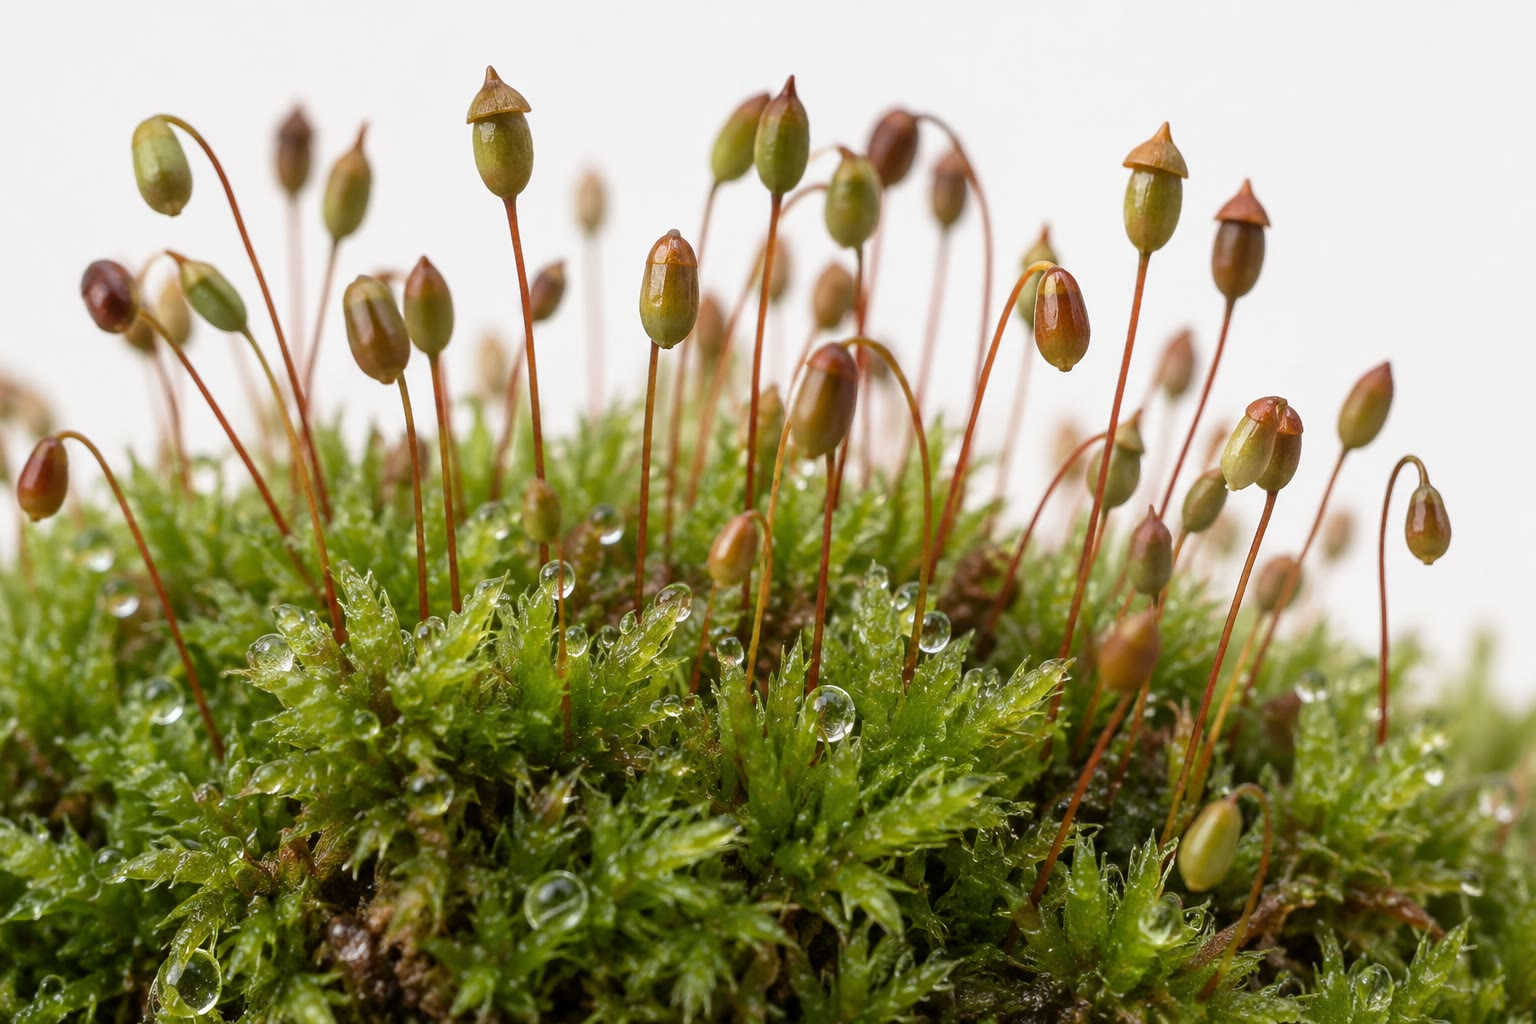
\includegraphics[width=0.6\linewidth]{images/book4/ai/b4-05-moss-sporophytes.jpg}

{\small Een moskussen in het voorjaar: de groene stengeltjes zijn de
\omterm{def:b2:plant-life-cycles:cycles}{gametofyten}, en elk roodachtig steeltje met zijn kapsel is een \omterm{def:b2:plant-life-cycles:cycles}{sporofyt}
die uit een bevruchte eicel is gegroeid, nog vast aan het stengeltje dat
de eicel maakte.}
\end{omfigure}

\begin{example}[De prijs van zwemmende zaadcellen]\label{ex:b2:plant-life-cycles:sperm}
Een zaadcel van een \omterm{def:b2:plant-life-cycles:moss}{mos} zwemt met ongeveer \qty{100}{\micro m/s}; om een
\omterm{def:b2:plant-life-cycles:moss}{archegonium} op \qty{2}{cm} afstand te bereiken, heeft ze \qty{200}{s}
ononderbroken waterfilm nodig --- een regenbui, een zware dauw. De
bevruchting is daardoor beperkt tot nat weer en tot korte afstanden, en
de meeste mossen, \omterm{def:b2:plant-life-cycles:fern}{varens} en hun verwanten leven op vochtige plaatsen of
planten zich in het natte seizoen voort; de antheridia van sommige
mossen zitten in een spatbekertje waarvan de vorm regendruppels, en de
zaadcellen die ze meevoeren, een halve meter ver slingert. Het is aan
deze afhankelijkheid dat de zaadplanten ontsnapten.
\end{example}

\section{Varens: de sporofyt is de plant}

\begin{definition}[De levenscyclus van een varen]\label{def:b2:plant-life-cycles:fern}
\index{varen}\index{prothallium}\index{sorus}\index{sporangium}
De varen is de \emph{\omterm{def:b2:plant-life-cycles:cycles}{sporofyt}}: een wortelstok met wortels, xyleem en
floëem, en bladeren. Aan de onderkant van vruchtbare bladeren maken
groepjes \emph{sporangia} (\emph{sori}, vaak onder een beschermend
dekvliesje) elk 64 sporen door \omterm{def:b2:meiosis-heredity:meiosis}{meiose}, die ze wegslingeren door het
openspringen van een uitdrogende ring van dikwandige cellen. Een spore
die op vochtige grond landt, groeit uit tot een \emph{prothallium}: een
hartvormige groene \omterm{def:b2:plant-life-cycles:cycles}{gametofyt} van enkele millimeters doorsnede, één cel
dik, met rizoïden, die enkele weken vrij leeft. Aan zijn onderkant
draagt hij antheridia en archegonia; zaadcellen zwemmen in de waterfilm
van de bodem naar de eicel; de zygote groeit uit tot een jonge \omterm{def:b2:plant-life-cycles:cycles}{sporofyt}
die zijn eerste voedsel uit het prothallium haalt en daarna wortel
schiet, waarna het prothallium sterft. De twee generaties zijn beide
zelfstandig, maar ongelijk: de \omterm{def:b2:plant-life-cycles:cycles}{sporofyt} leeft tientallen jaren en kan
meters hoog worden, de \omterm{def:b2:plant-life-cycles:cycles}{gametofyt} leeft weken en meet millimeters.
\end{definition}

\begin{omfigure}
\begin{tikzpicture}[every node/.style={font=\scriptsize}, >=stealth]
  \node[draw, rounded corners, fill=omThm!12, align=center] (fern) at (0,3) {varenplant, de sporofyt ($2n$)\\wortels, wortelstok, bladeren};
  \node[draw, rounded corners, fill=omThm!12, align=center] (sor) at (5.4,3) {sporangia in sori\\(onder de bladeren)};
  \node[draw, rounded corners, fill=omDef!12, align=center] (spore) at (10.4,3) {sporen ($n$)\\64 per sporangium};
  \node[draw, rounded corners, fill=omDef!12, align=center] (pro) at (10.4,0.6) {prothallium ($n$)\\vrijlevend, mm-groot\\antheridia, archegonia};
  \node[draw, rounded corners, fill=omDef!12, align=center] (gam) at (5.4,0.6) {zaadcel en eicel ($n$)};
  \node[draw, rounded corners, fill=omThm!12, align=center] (zyg) at (0,0.6) {zygote ($2n$), daarna\\jonge sporofyt\\op het prothallium};
  \draw[->, thick] (fern) -- (sor);
  \draw[->, thick] (sor) -- (spore) node[midway, above] {meiose};
  \draw[->, thick] (spore) -- (pro) node[midway, right] {mitose};
  \draw[->, thick] (pro) -- (gam) node[midway, above] {mitose};
  \draw[->, thick] (gam) -- (zyg) node[midway, above, align=center] {bevruchting\\(zwemmende zaadcellen)};
  \draw[->, thick] (zyg) -- (fern) node[midway, right] {mitose};
  \draw[gray, dashed] (7.9,-0.5) -- (7.9,4.0);
  \node[omThm, anchor=south] at (2.7,3.9) {diploïde generatie};
  \node[omDef, anchor=south] at (10.4,3.9) {haploïde generatie};
\end{tikzpicture}

{\small De cyclus van een \omterm{def:b2:plant-life-cycles:fern}{varen}. De plant die men een \omterm{def:b2:plant-life-cycles:fern}{varen} noemt, is de
diploïde \omterm{def:b2:plant-life-cycles:cycles}{sporofyt}; de haploïde \omterm{def:b2:plant-life-cycles:cycles}{gametofyt} is een kortlevend \omterm{def:b2:plant-life-cycles:fern}{prothallium}
waarop de zaadcellen naar de eicellen zwemmen.}
\end{omfigure}

\begin{omfigure}
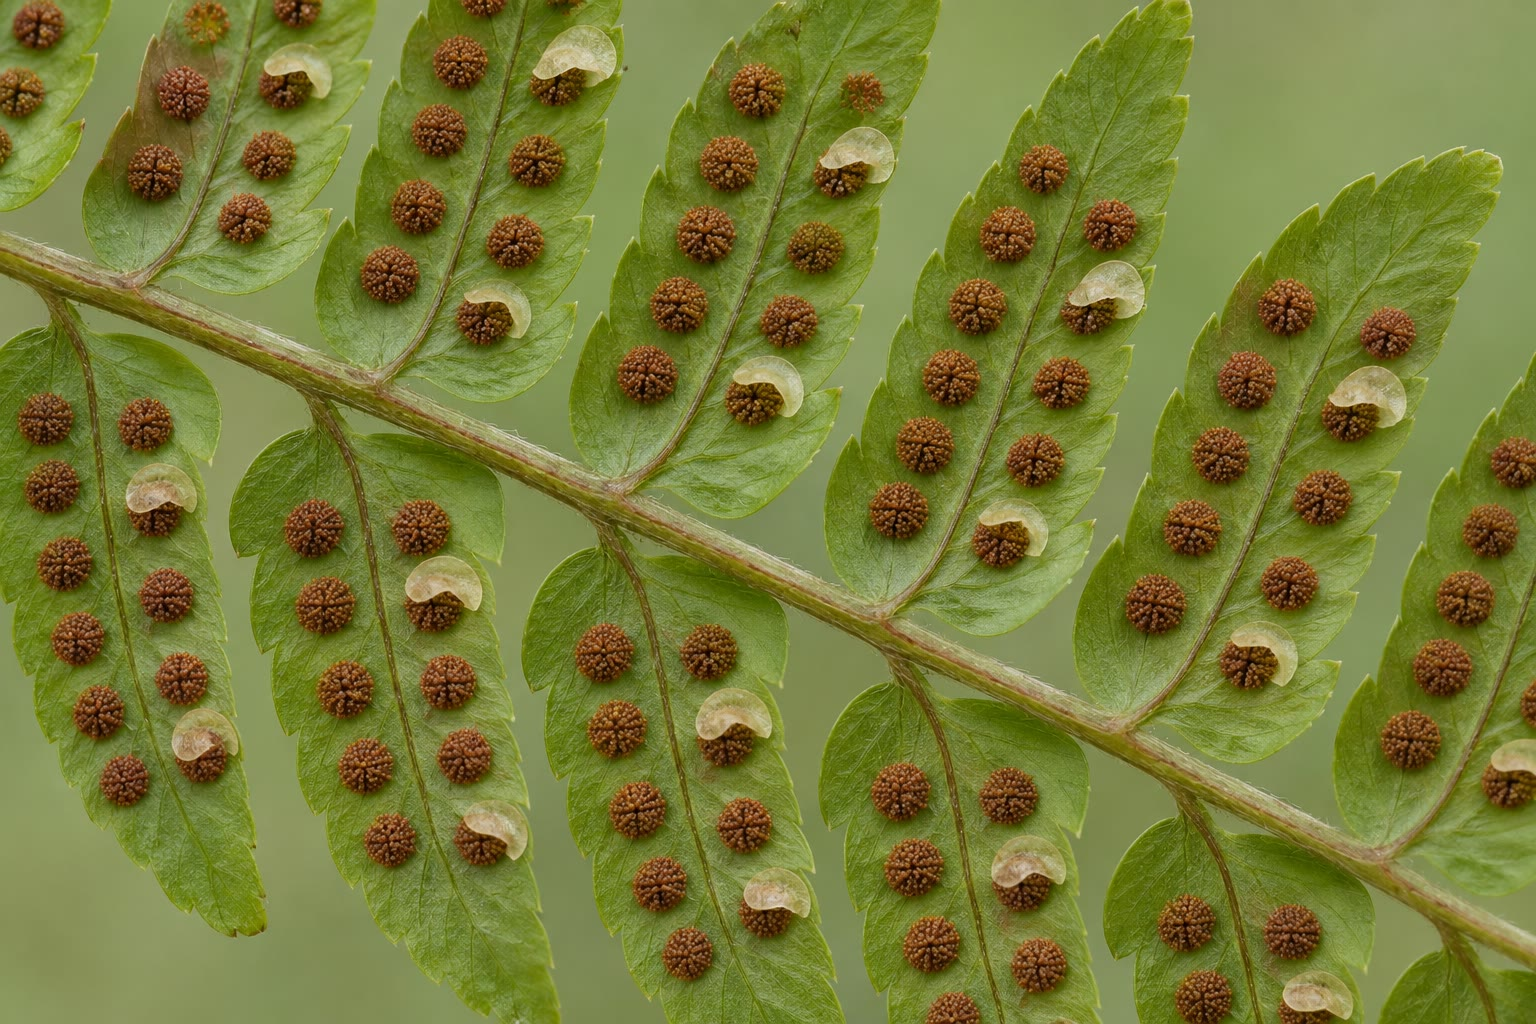
\includegraphics[width=0.6\linewidth]{images/book4/ai/b4-05-fern-sori.jpg}

{\small De onderkant van een vruchtbaar varenblad: elk bruin stipje is een
\omterm{def:b2:plant-life-cycles:fern}{sorus}, een groepje sporangia, sommige nog bedekt door het dekvliesje dat
ze beschermt tot ze rijp zijn.}
\end{omfigure}

\begin{theorem}[Verspreiding van een spore]\label{thm:b2:plant-life-cycles:dispersal}
\index{verspreiding van sporen}
Een spore met straal $r$ en dichtheid $\rho_s$ die op hoogte $h$ wordt
losgelaten in een horizontale wind met snelheid $u$, valt met de
eindsnelheid van Stokes
$v_s = 2r^2(\rho_s - \rho_{\text{lucht}})g/9\eta_{\text{lucht}}$
en landt, in gelaagde stilstaande lucht, op een afstand
\[
x = \frac{u\,h}{v_s}
\]
van de plant. Een varenspore met straal \qty{15}{\micro m} en
dichtheid \qty{1100}{kg/m^3} ($\eta_{\text{lucht}} = \qty{1.8e-5}{Pa.s}$)
valt met \qty{3}{cm/s}; vanaf een blad op \qty{0.5}{m} legt ze in een
wind van \qty{2}{m/s} ongeveer \qty{30}{m} af, en in de turbulente lucht
van een winderige dag, die een deel van de sporen hoog boven de
loslaathoogte optilt, reizen er enkele honderden kilometers --- en daarom
zijn de varenflora's van oceanische eilanden rijk en hun flora's van
zaadplanten arm.
\end{theorem}
\begin{proof}
De valtijd is $h/v_s$ (de spore bereikt haar eindsnelheid in
microseconden), en in die tijd voert de wind haar $u\,h/v_s$ mee. De
eindsnelheid volgt uit het evenwicht tussen de wrijvingskracht van Stokes $6\pi\eta r
v_s$ en het gewicht min de opwaartse kracht $\tfrac43\pi r^3(\rho_s -
\rho_{\text{lucht}})g$, zoals in \cref{ch:b2:unicellular-diversity}.
\end{proof}

\section{Zaadplanten: de gametofyt is verborgen}

\begin{definition}[Heterosporie, stuifmeel, zaadbeginsel]\label{def:b2:plant-life-cycles:heterospory}
\index{heterosporie}\index{stuifmeel}\index{zaadbeginsel}\index{microspore}\index{megaspore}
Mossen en de meeste \omterm{def:b2:plant-life-cycles:fern}{varens} zijn \emph{isospoor}: één soort spore, één
soort \omterm{def:b2:plant-life-cycles:cycles}{gametofyt} die beide geslachten draagt. Zaadplanten (en enkele
\omterm{def:b2:plant-life-cycles:fern}{varens} en wolfsklauwen) zijn \emph{heterospoor}: \emph{microsporen},
klein en talrijk, groeien uit tot mannelijke \omterm{def:b2:plant-life-cycles:cycles}{gametofyten};
\emph{megasporen}, groot en weinig talrijk, tot vrouwelijke. Bij
zaadplanten zijn beide tot bijna niets teruggebracht en verlaat geen van
beide op eigen kracht de weefsels van de \omterm{def:b2:plant-life-cycles:cycles}{sporofyt}. De mannelijke
\omterm{def:b2:plant-life-cycles:cycles}{gametofyt} is de \emph{stuifmeelkorrel}: een microspore die zich binnen
haar wand twee of drie keer heeft gedeeld, door wind of dieren naar het
vrouwelijke orgaan gebracht, waar ze een \emph{stuifmeelbuis} vormt en
haar zaadcellen afgeeft --- zonder water. De vrouwelijke \omterm{def:b2:plant-life-cycles:cycles}{gametofyt}
ontwikkelt zich in het megasporangium, dat op de ouderplant blijft,
omsloten door een of twee \emph{integumenten} met een opening, de
\emph{micropyle}: de hele structuur is het \emph{zaadbeginsel}. Na de
bevruchting wordt het zaadbeginsel het \emph{zaad}: een embryonale
\omterm{def:b2:plant-life-cycles:cycles}{sporofyt}, een voedselvoorraad en een zaadhuid, gevormd uit de
integumenten, in rust tot de omstandigheden gunstig zijn.
\end{definition}

\begin{omfigure}
\begin{tikzpicture}[every node/.style={font=\scriptsize}]
  % ovule in section
  \draw[thick, fill=omExo!25] (0,0) ellipse (1.6 and 2.2);
  \draw[thick, fill=omExo!10] (0,0) ellipse (1.25 and 1.85);
  \draw[thick, fill=white] (0,-0.15) ellipse (0.8 and 1.3);
  \draw[thick, fill=omDef!25] (0,0.6) ellipse (0.45 and 0.55);
  \fill[omDef!80!black] (0,0.75) circle (0.12);
  % micropyle: gap at top
  \fill[white] (-0.35,1.7) rectangle (0.35,2.35);
  \draw[thick] (-0.35,1.7) -- (-0.35,2.2); \draw[thick] (0.35,1.7) -- (0.35,2.2);
  \draw[thick] (-0.35,2.2) arc (180:90:0.1) ; \draw[thick] (0.35,2.2) arc (0:90:0.1);
  % pollen grain and tube
  \draw[thick, fill=omProp!40] (0.9,3.0) circle (0.22);
  \draw[thick, omProp] (0.75,2.85) .. controls (0.2,2.6) and (0.05,2.0) .. (0.05,1.25);
  % stalk
  \draw[thick] (0,-2.2) -- (0,-2.8);
  % labels
  \draw (1.45,-0.9) -- (2.6,-0.9) node[right] {integument(en)};
  \draw (1.0,-0.6) -- (2.6,-1.5) node[right] {megasporangium (nucellus)};
  \draw (0.55,-1.0) -- (2.6,-2.1) node[right, align=left] {vrouwelijke gametofyt\\(uit één megaspore)};
  \draw (0.35,0.45) -- (2.6,0.3) node[right] {archegonium};
  \draw (0.1,0.78) -- (2.6,1.0) node[right] {eicel};
  \draw (0.35,2.0) -- (2.6,2.0) node[right] {micropyle};
  \draw (1.1,3.0) -- (2.6,3.0) node[right] {stuifmeelkorrel en stuifmeelbuis};
  \node[right] at (0.1,-2.6) {steel};
\end{tikzpicture}

{\small Een \omterm{def:b2:plant-life-cycles:heterospory}{zaadbeginsel} van een naaktzadige in doorsnede. De vrouwelijke
\omterm{def:b2:plant-life-cycles:cycles}{gametofyt}, gegroeid uit één \omterm{def:b2:plant-life-cycles:heterospory}{megaspore} in het megasporangium, is omhuld
door een integument met een opening; de stuifmeelkorrel, opgevangen bij
de micropyle, groeit met een buis naar de eicel. Na de bevruchting wordt
het geheel het zaad.}
\end{omfigure}

\begin{proposition}[De cyclus van een conifeer]\label{prop:b2:plant-life-cycles:conifer}
\index{conifeer}\index{kegel}\index{zaad}
Een den draagt twee soorten kegels. Kleine \emph{mannelijke kegels}, in
het voorjaar in trossen, bevatten microsporangia waarin de \omterm{def:b2:meiosis-heredity:meiosis}{meiose}
\omterm{def:b2:plant-life-cycles:heterospory}{microsporen} maakt; elke \omterm{def:b2:plant-life-cycles:heterospory}{microspore} deelt zich tot een viercellige
stuifmeelkorrel met twee luchtzakken, die bij miljoenen in de wind wordt
uitgestrooid. \emph{Vrouwelijke kegels} dragen op de bovenzijde van elke
schub twee \omterm{def:b2:plant-life-cycles:heterospory}{zaadbeginsels}. \omterm{def:b2:plant-life-cycles:heterospory}{Stuifmeel} dat tussen de schubben waait, wordt
door een druppel vocht naar de micropyle getrokken; de vrouwelijke
\omterm{def:b2:plant-life-cycles:cycles}{gametofyt}, die zich nog niet heeft ontwikkeld, groeit dan in de loop van
het volgende jaar uit de enige overlevende \omterm{def:b2:plant-life-cycles:heterospory}{megaspore} uit tot een weefsel
van enkele duizenden cellen met twee of drie archegonia; een
stuifmeelbuis groeit langzaam door de nucellus en brengt vijftien
maanden na de bestuiving een zaadcel naar een eicel. Het embryo
ontwikkelt zich in de \omterm{def:b2:plant-life-cycles:cycles}{gametofyt}, die de voedselvoorraad van het zaad
wordt; het gevleugelde zaad wordt in de tweede herfst uitgestrooid,
wanneer de kegel opengaat. Zaden vergen jaren en kosten veel; in ruil
worden ze droog verspreid, overleven ze winter en droogte, en dragen ze
het voedsel voor de eerste weken van de kiemplant mee.
\end{proposition}

\begin{omfigure}
\begin{tikzpicture}[every node/.style={font=\scriptsize}, >=stealth]
  \draw[thick, ->] (0,0) -- (13.2,0);
  \foreach \x/\l in {0/{voorjaar, jaar 1}, 4.4/{voorjaar, jaar 2}, 8.8/{herfst, jaar 2}, 12.4/{}}
    \draw (\x,0.1) -- (\x,-0.1) node[below] {\l};
  \node[above, align=center, omProp] at (0.6,0.3) {bestuiving:\\stuifmeel opgevangen bij de micropyle};
  \node[above, align=center, omDef] at (3.0,1.2) {vrouwelijke gametofyt groeit\\uit de megaspore (een jaar)};
  \draw[omDef, thick] (0.8,1.15) -- (5.2,1.15);
  \node[above, align=center, omThm] at (5.6,0.3) {bevruchting:\\stuifmeelbuis bereikt de eicel};
  \node[above, align=center, omThm] at (8.2,1.2) {embryo ontwikkelt zich\\in de gametofyt};
  \draw[omThm, thick] (5.8,1.15) -- (10.4,1.15);
  \node[above, align=center] at (10.8,0.3) {kegel gaat open:\\gevleugelde zaden vallen};
\end{tikzpicture}

{\small Het tijdschema van een dennenzaad: bestuiving in het eerste
voorjaar, bevruchting meer dan een jaar later, uitstrooien van het zaad
in de tweede herfst --- ongeveer achttien maanden van \omterm{def:b2:plant-life-cycles:heterospory}{stuifmeel} tot zaad.}
\end{omfigure}

\begin{omfigure}
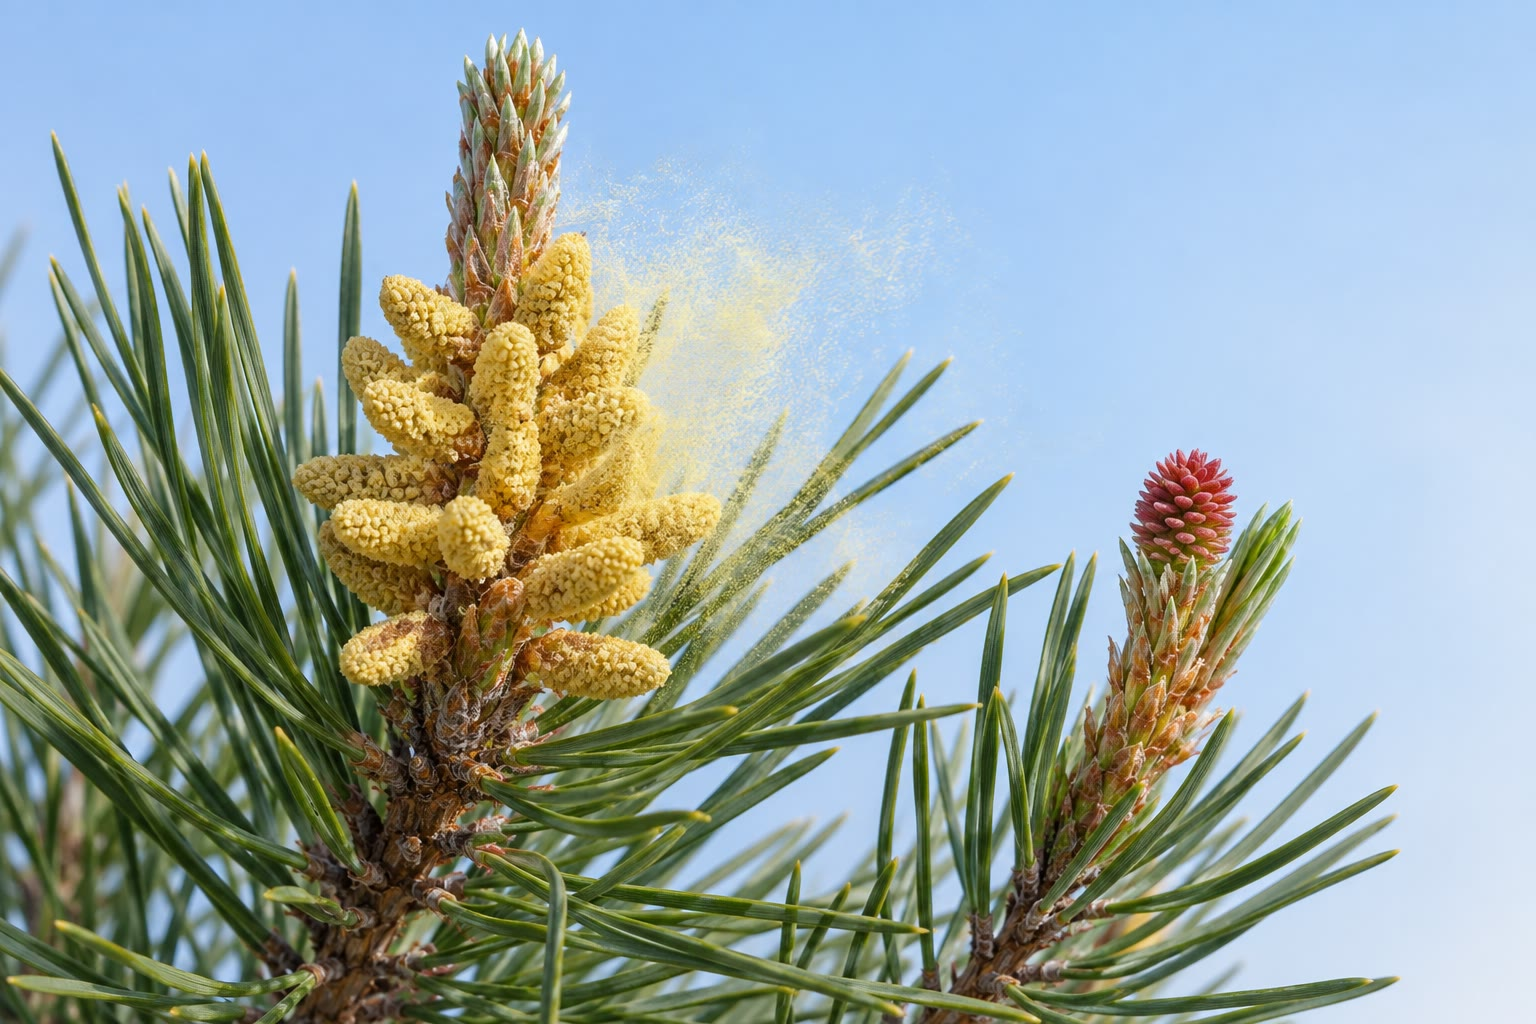
\includegraphics[width=0.6\linewidth]{images/book4/ai/b4-05-pine-cones.jpg}

{\small Een dennentak in het voorjaar: een tros gele mannelijke kegels die
\omterm{def:b2:plant-life-cycles:heterospory}{stuifmeel} uitstrooien, en een kleine rode vrouwelijke kegel aan de top van
een andere tak, met open schubben om het op te vangen.}
\end{omfigure}

\begin{example}[Stuifmeel in de wind]\label{ex:b2:plant-life-cycles:pollen}
Een stuifmeelkorrel van een den, \qty{50}{\micro m} groot en met twee
luchtzakken, valt met ongeveer \qty{3}{cm/s}; een grote boom laat in een
seizoen zo'n $10^{11}$ korrels los, genoeg om vijvers geel te kleuren. De
kans dat één korrel op een bepaald \omterm{def:b2:plant-life-cycles:heterospory}{zaadbeginsel} landt, is piepklein, en
de strategie werkt alleen in grote aantallen: windbestuiving is goedkoop
per korrel, duur in korrels, en beperkt tot planten die in bestanden van
hun eigen soort groeien --- coniferen, grassen, eiken. De bloemplanten
(\cref{ch:b2:angiosperm-reproduction}) vonden een manier om \omterm{def:b2:plant-life-cycles:heterospory}{stuifmeel}
door dieren te laten bezorgen, korrel voor korrel op het juiste adres.
\end{example}

\section{Trends bij de landplanten}

\begin{proposition}[Vier trends]\label{prop:b2:plant-life-cycles:trends}
\index{reductie van de gametofyt}
Van mossen via \omterm{def:b2:plant-life-cycles:fern}{varens} naar zaadplanten: (1) de \omterm{def:b2:plant-life-cycles:cycles}{sporofyt} groeit van een
afhankelijk steeltje uit tot de hele plant, en de \omterm{def:b2:plant-life-cycles:cycles}{gametofyt} krimpt van de
plant tot een schubje tot enkele cellen; (2) isosporie maakt plaats voor
\omterm{def:b2:plant-life-cycles:heterospory}{heterosporie}, en de vrouwelijke \omterm{def:b2:plant-life-cycles:cycles}{gametofyt} blijft op de ouderplant;
(3) de bevruchting gaat van zwemmende zaadcellen in oppervlaktewater over
op een stuifmeelbuis, zodat de voortplanting geen regen meer nodig heeft;
(4) de verspreidingseenheid gaat van de spore --- één cel met reserves
voor een dag --- over op het zaad, een embryo met voedsel en een
zaadhuid, dat kan wachten. De diploïde generatie wordt op het land
begunstigd, omdat een \omterm{def:b2:meiosis-heredity:meiosis}{diploïd} lichaam recessieve \omterm{def:b2:genome-diversification:mutation}{mutaties} maskeert, met
een vaatstelsel groter en langlevender kan worden, en omdat een spore die
door \omterm{def:b2:meiosis-heredity:meiosis}{meiose} op een hoge \omterm{def:b2:plant-life-cycles:cycles}{sporofyt} wordt gemaakt verder reist dan een gameet
die van een lage \omterm{def:b2:plant-life-cycles:cycles}{gametofyt} wegzwemt. De trend zet zich voort bij de
bloemplanten, waar de vrouwelijke \omterm{def:b2:plant-life-cycles:cycles}{gametofyt} zeven cellen telt en het zaad
in een vrucht is gewikkeld.
\end{proposition}

\begin{example}[De groepen vergeleken]\label{ex:b2:plant-life-cycles:table}
\begin{center}
\small
\begin{tabular}{p{2.3cm}p{3.1cm}p{3.1cm}p{3.3cm}}
\hline
 & mossen & \omterm{def:b2:plant-life-cycles:fern}{varens} & coniferen \\
\hline
dominante generatie & \omterm{def:b2:plant-life-cycles:cycles}{gametofyt} & \omterm{def:b2:plant-life-cycles:cycles}{sporofyt} & \omterm{def:b2:plant-life-cycles:cycles}{sporofyt} \\
\omterm{def:b2:plant-life-cycles:cycles}{gametofyt} & bebladerd stengeltje, cm & \omterm{def:b2:plant-life-cycles:fern}{prothallium}, mm, vrij & stuifmeelkorrel (4 cellen); inhoud van het \omterm{def:b2:plant-life-cycles:heterospory}{zaadbeginsel} (duizenden cellen) \\
sporen & één soort & één soort & \omterm{def:b2:plant-life-cycles:heterospory}{microsporen}, \omterm{def:b2:plant-life-cycles:heterospory}{megasporen} \\
bevruchting & zaadcellen zwemmen in water & zaadcellen zwemmen in water & stuifmeelbuis \\
verspreiding & spore & spore & zaad \\
vaatweefsel & geen & xyleem, floëem & xyleem, floëem, hout \\
\hline
\end{tabular}
\end{center}
\end{example}

\section{Opgaven}

\begin{exercise}[$\star$]\label{exo:b2:plant-life-cycles:1}
Definieer \omterm{def:b2:plant-life-cycles:cycles}{gametofyt}, \omterm{def:b2:plant-life-cycles:cycles}{sporofyt}, spore en gameet, en zeg door welk soort
deling (mitose of \omterm{def:b2:meiosis-heredity:meiosis}{meiose}) elk van de vier wordt gevormd.
\end{exercise}

\begin{exercise}[$\star$]\label{exo:b2:plant-life-cycles:2}
De \omterm{def:b2:plant-life-cycles:fern}{varen} \emph{Ophioglossum reticulatum} heeft \num{1260}
chromosomen in zijn bladcellen. Hoeveel zijn het er in een spore, een
cel van het \omterm{def:b2:plant-life-cycles:fern}{prothallium}, een zaadcel, een eicel, een zygote?
\end{exercise}

\begin{exercise}[$\star$]\label{exo:b2:plant-life-cycles:3}
Welke generatie is het groene kussen van een \omterm{def:b2:plant-life-cycles:moss}{mos}? Het bruine steeltje
met een kapsel? Een varenblad? Een \omterm{def:b2:plant-life-cycles:fern}{prothallium}? Een stuifmeelkorrel? De
voedselvoorraad van een dennenzaad? Het embryo van een dennenzaad?
\end{exercise}

\begin{exercise}[$\star$]\label{exo:b2:plant-life-cycles:4}
Noem de drie soorten \omterm{def:b2:plant-life-cycles:cycles}{levenscyclus} en geef bij elk een organisme.
Waar vindt bij elk de \omterm{def:b2:meiosis-heredity:meiosis}{meiose} plaats?
\end{exercise}

\begin{exercise}[$\star\star$]\label{exo:b2:plant-life-cycles:5}
Een zaadcel van een \omterm{def:b2:plant-life-cycles:moss}{mos} zwemt met \qty{100}{\micro m/s}. Hoelang doet ze
erover om een \omterm{def:b2:plant-life-cycles:moss}{archegonium} op \qty{3}{cm} afstand te bereiken? Een
dauwfilm verdampt \qty{20}{min} na zonsopgang: wat is het maximale bereik
van de bevruchting? Becommentarieer de grootte van moskolonies.
\end{exercise}

\begin{exercise}[$\star\star$]\label{exo:b2:plant-life-cycles:6}
Bereken de valsnelheid in lucht van een varenspore met straal
\qty{15}{\micro m} en dichtheid \qty{1100}{kg/m^3} ($\eta =
\qty{1.8e-5}{Pa.s}$, $\rho_{\text{lucht}} = \qty{1.2}{kg/m^3}$), en
de afstand die ze vanaf \qty{0.5}{m} aflegt in een wind van \qty{2}{m/s}.
Doe hetzelfde voor een dennenzaad met massa \qty{5}{mg} waarvan de vleugel
een daalsnelheid van \qty{0.8}{m/s} geeft, losgelaten op \qty{20}{m}.
\end{exercise}

\begin{exercise}[$\star\star$]\label{exo:b2:plant-life-cycles:7}
Een varenblad draagt \num{200} sori van \num{40} sporangia, en elk
\omterm{def:b2:plant-life-cycles:fern}{sporangium} maakt \num{64} sporen. Hoeveel sporen per blad? Als
één spore op $10^{5}$ een \omterm{def:b2:plant-life-cycles:fern}{prothallium} wordt en één \omterm{def:b2:plant-life-cycles:fern}{prothallium} op
\num{50} een \omterm{def:b2:plant-life-cycles:cycles}{sporofyt} voortbrengt, hoeveel jonge \omterm{def:b2:plant-life-cycles:fern}{varens} levert een blad
dan op?
\end{exercise}

\begin{exercise}[$\star\star$]\label{exo:b2:plant-life-cycles:8}
Leg uit waarom \omterm{def:b2:plant-life-cycles:heterospory}{heterosporie} een voorwaarde is voor het zaad, en waarom
een isospore plant haar vrouwelijke \omterm{def:b2:plant-life-cycles:cycles}{gametofyt} niet in een \omterm{def:b2:plant-life-cycles:heterospory}{zaadbeginsel}
zou kunnen insluiten.
\end{exercise}

\begin{exercise}[$\star\star$]\label{exo:b2:plant-life-cycles:9}
Vergelijk een varenspore (een bol met straal \qty{15}{\micro m}, dichtheid
\qty{1100}{kg/m^3}) en een dennenzaad (\qty{5}{mg}) als
verspreidingseenheden: massa, energie-inhoud (neem \qty{20}{kJ/g} droge
stof, \qty{50}{\%} droog), en wat elk bij het landen wel en niet kan.
\end{exercise}

\begin{exercise}[$\star\star\star$]\label{exo:b2:plant-life-cycles:10}
Een den laat $10^{11}$ stuifmeelkorrels los boven een bos; op de hoogte
van de \omterm{def:b2:plant-life-cycles:heterospory}{zaadbeginsels} zijn de korrels verdeeld over een laag van
\qty{20}{m} dik boven \qty{1}{km^2}. Schat de stuifmeelconcentratie
(korrels per kubieke meter), het aantal korrels per seconde dat in een
wind van \qty{2}{m/s} door de opening bij de micropyle van een
\omterm{def:b2:plant-life-cycles:heterospory}{zaadbeginsel} (\qty{0.1}{mm^2}) gaat, en de tijd die een \omterm{def:b2:plant-life-cycles:heterospory}{zaadbeginsel}
nodig heeft om één korrel te ontvangen. Wat zegt dit over het tijdstip
waarop de kegels opengaan?
\end{exercise}

\begin{exercise}[$\star\star\star$]\label{exo:b2:plant-life-cycles:11}
Geef drie redenen waarom de diploïde generatie in de \omterm{def:b2:plant-life-cycles:cycles}{levenscyclus} van
landplanten ging overheersen, en één reden waarom de haploïde generatie
niet helemaal verdween.
\end{exercise}

\begin{exercise}[$\star\star\star$]\label{exo:b2:plant-life-cycles:12}
Hofmeister werkte voordat chromosomen bekend waren. Leg uit wat hij
alleen met microscopie en kweek over de \omterm{def:b2:plant-life-cycles:cycles}{generatiewisseling} kon vaststellen
en wat niet, en wat de chromosoomtellingen daaraan toevoegden.
\end{exercise}

\section{Vraagstuk: van spore tot zaad}

\begin{problem}[{Weekendvraagstuk --- de voortplantingsrekensom van een
varen en een den vergeleken, van het aantal sporen en stuifmeelkorrels
tot hun verspreiding, het lot van de gametofyten en de kosten van een
zaad, met als besluit het aantal verspreidingseenheden dat elke plant
moet maken voor één vervanger}]
\label{pb:b2:plant-life-cycles:1}
Een varenplant draagt \num{10} vruchtbare bladeren, elk met \num{200}
sori van \num{40} sporangia die elk \num{64} sporen maken. Sporen:
straal \qty{15}{\micro m}, dichtheid \qty{1100}{kg/m^3}. Een den
produceert in zijn leven de \omterm{def:b2:plant-life-cycles:heterospory}{zaadbeginsels} van $2\times 10^{4}$ vrouwelijke
kegels --- neem \num{100} \omterm{def:b2:plant-life-cycles:heterospory}{zaadbeginsels} per kegel --- en $10^{11}$
stuifmeelkorrels per jaar. Zaden: \qty{5}{mg}, \qty{50}{\%} droge stof à
\qty{20}{kJ/g}. Lucht: $\eta = \qty{1.8e-5}{Pa.s}$, $\rho =
\qty{1.2}{kg/m^3}$; $g = \qty{9.81}{m/s^2}$.

\medskip
\noindent\textbf{Deel I --- De sporen van de \omterm{def:b2:plant-life-cycles:fern}{varen}.}
\begin{enumerate}
  \item Bereken het aantal sporen dat de plant in een seizoen uitstrooit.
  \item Bereken de massa van één spore en van de hele oogst.
  \item Bereken de valsnelheid van de spore in lucht.
  \item Hoe ver reizen de sporen vanaf bladeren op \qty{0.5}{m} in een
        wind van \qty{1.5}{m/s}? Over hoe groot een oppervlak (een schijf
        met die straal) worden ze verspreid, en hoeveel landen er per
        vierkante meter?
  \item Leg uit waarom turbulentie enkele sporen veel verder draagt, en
        wat dit betekent voor de kolonisatie van een nieuw eiland.
  \item Bereken de energie-inhoud van één spore (\qty{50}{\%} droge stof
        à \qty{20}{kJ/g}) en van de hele oogst, en vergelijk met de energie
        van één dennenzaad.
\end{enumerate}

\medskip
\noindent\textbf{Deel II --- De \omterm{def:b2:plant-life-cycles:cycles}{gametofyten}.}
Eén spore op $2\times 10^{4}$ landt op grond die vochtig genoeg is om tot
een \omterm{def:b2:plant-life-cycles:fern}{prothallium} uit te groeien; een \omterm{def:b2:plant-life-cycles:fern}{prothallium} leeft \num{6} weken en
heeft voor de bevruchting een natte nacht nodig --- kans $0.2$ per week;
een bevrucht \omterm{def:b2:plant-life-cycles:fern}{prothallium} geeft met kans
$0.5$ een jonge \omterm{def:b2:plant-life-cycles:cycles}{sporofyt}; een jonge \omterm{def:b2:plant-life-cycles:cycles}{sporofyt} overleeft tot volwassenheid
met kans
$0.02$.
\begin{enumerate}[resume]
  \item Hoeveel prothallia levert de oogst van de plant op?
  \item Bereken de kans dat een \omterm{def:b2:plant-life-cycles:fern}{prothallium} in zijn zes weken minstens
        één natte nacht meemaakt.
  \item Bereken het verwachte aantal volwassen \omterm{def:b2:plant-life-cycles:fern}{varens} dat de oogst van
        één seizoen oplevert.
  \item Als de ouderplant \num{30} jaar leeft, hoeveel volwassen
        nakomelingen laat hij dan na, en wat zegt dit over de
        varenpopulatie?
  \item Een zaadcel zwemt, zoals bij mossen, met \qty{100}{\micro m/s},
        en de archegonia van een \omterm{def:b2:plant-life-cycles:fern}{prothallium} liggen op \qty{1}{mm} van
        zijn eigen antheridia. Hoelang duurt zelfbevruchting? Waarom
        vermijden veel \omterm{def:b2:plant-life-cycles:fern}{varens} die toch (geef één mechanisme)?
  \item In welke zin is het \omterm{def:b2:plant-life-cycles:fern}{prothallium} de zwakke schakel van de cyclus
        van de \omterm{def:b2:plant-life-cycles:fern}{varen}?
\end{enumerate}

\medskip
\noindent\textbf{Deel III --- Het \omterm{def:b2:plant-life-cycles:heterospory}{stuifmeel} van de den.}
\begin{enumerate}[resume]
  \item Een stuifmeelkorrel is een bol met straal \qty{25}{\micro m} en een
        effectieve dichtheid van \qty{600}{kg/m^3} (luchtzakken
        inbegrepen). Bereken zijn valsnelheid.
  \item Hoe ver reist hij vanaf een kegel op \qty{15}{m} in een wind van
        \qty{3}{m/s}?
  \item De $10^{11}$ korrels worden verdeeld over \qty{1}{km^2} bos tot
        een diepte van \qty{20}{m}. Bereken de concentratie.
  \item Een micropyle biedt een opening van \qty{0.1}{mm^2} aan een wind
        van \qty{2}{m/s}. Bereken het aantal korrels dat er per uur
        binnenkomt, en de tijd tot de eerste korrel.
  \item Leg uit waarom een alleenstaande den op \qty{5}{km} van het bos
        vrijwel geen zaad zet, en waarom windbestoven soorten in
        bestanden groeien.
  \item Vergelijk de aantallen: hoeveel stuifmeelkorrels maakt het bos
        per \omterm{def:b2:plant-life-cycles:heterospory}{zaadbeginsel}, als het \num{1000} dennen met elk \num{2000}
        \omterm{def:b2:plant-life-cycles:heterospory}{zaadbeginsels} telt?
\end{enumerate}

\medskip
\noindent\textbf{Deel IV --- De zaden van de den.}
Van de \omterm{def:b2:plant-life-cycles:heterospory}{zaadbeginsels} van de boom wordt \qty{60}{\%} bestoven en daarvan
vormt \qty{80}{\%} een zaad; een zaad wordt met kans $0.05$ een kiemplant
en een kiemplant met kans $0.01$ een volwassen boom.
\begin{enumerate}[resume]
  \item Bereken het aantal zaden dat de boom in zijn leven maakt, en hun
        totale massa en energie.
  \item Een gevleugeld zaad daalt met \qty{0.8}{m/s}. Hoe ver reist het
        vanaf \qty{20}{m} in een wind van \qty{3}{m/s}? Vergelijk met het
        \omterm{def:b2:plant-life-cycles:heterospory}{stuifmeel}.
  \item Bereken het verwachte aantal volwassen nakomelingen, en vergelijk
        met dat van de \omterm{def:b2:plant-life-cycles:fern}{varen}.
  \item Bereken de energie die de boom per volwassen nakomeling investeert,
        en die van de \omterm{def:b2:plant-life-cycles:fern}{varen} per volwassen nakomeling (alleen sporen), en
        vergelijk.
  \item De varenspore kan enkele weken wachten; het dennenzaad
        verscheidene jaren. Leg met de energiecijfers uit waarom het zaad
        zich een rustperiode kan veroorloven en de spore niet.
  \item Geef twee voordelen die het zaad zijn kosten waard maken en twee
        omstandigheden waarin de strategie van de \omterm{def:b2:plant-life-cycles:fern}{varen} de betere is.
  \item Formuleer het resultaat: verspreidingseenheden per volwassen
        nakomeling voor de \omterm{def:b2:plant-life-cycles:fern}{varen} en voor de den, en de energie die elk per
        volwassen nakomeling besteedt.
\end{enumerate}
\end{problem}
